\documentclass[12pt]{article}
%Gummi|065|=)
\usepackage{amsmath, amsfonts, amssymb}
\usepackage[margin=0.5in]{geometry}
\usepackage{xcolor}
\usepackage{graphicx}

\newcommand{\off}[1]{}
\DeclareMathSizes{20}{30}{20}{18}

\newcommand{\two }{\sqrt[3]{2}}
\newcommand{\four}{\sqrt[3]{4}}
\newcommand{\red}{\begin{tikz}[scale=0.25]
\draw[fill=red, color=red] (0,0)--(1,0)--(1,1)--(0,1)--cycle;\end{tikz}}
\newcommand{\blue}{\begin{tikz}[scale=0.25]
\draw[fill=blue, color=blue] (0,0)--(1,0)--(1,1)--(0,1)--cycle;\end{tikz}}
\newcommand{\green}{\begin{tikz}[scale=0.25]
\draw[fill=green, color=green] (0,0)--(1,0)--(1,1)--(0,1)--cycle;\end{tikz}}

\newcommand{\sq}[3]{\draw[#3] (#1,#2)--(#1+1,#2)--(#1+1,#2+1)--(#1,#2+1)--cycle;}

\usepackage{tikz}

\newcommand{\susy}{{\bf Q}}
\newcommand{\RV}{{\text{R}_\text{V}}}

\title{Worksheet: Markoff Triples}
\author{John D Mangual}
\date{}
\begin{document}

\fontfamily{qag}\selectfont \fontsize{12.5}{15}\selectfont

\maketitle

\noindent Politically, let's see what modern number theorists are doing.  At least initiall, it's kid stuff.  And when you follow it through it still feels like GH Hardy, with some extra stuff.   \\ \\ \\
Sarnak has been leading some discussion of the Markoff triples.  I'll start with what I know. And then see how he put it in context.
$$ q || q \theta || <  5^{-\tfrac{1}{2}} $$
This equation has infinitely many integer solutions $q \in \mathbb{Z}$.  This is the best we can do in case:
$$ \theta^2 - \theta + 1 = 0 $$
The next one down the line:
$$ q || q \theta || <  2^{-\tfrac{3}{2}} $$
This equation has infinitely many integer solutions $q \in \mathbb{Z}$.  This is the best we can do in case:
$$ \theta^2 +2\theta - 1 = 0 $$
Otherwise there are infinitely many solutions of:
$$ q || q \theta || <  5/221^{-\tfrac{1}{2}} $$
This equation has infinitely many integer solutions $q \in \mathbb{Z}$.  This is the best we can do in case:
$$ 5\theta^2 + 11\theta - 5 = 0 $$
This is (confusingly) called the \textbf{Markov chain} and somehow this is related to the Markov diophantine equation $ a^2 + b^2 + c^2  = 3abc $.  There is a descent:
$$ (a,b,c) \mapsto ( bc - a , b, c) $$
and we could build an entire ``tree" of solutions this way\dots \\ \\ \\
We could ask about strong approximation.  And we know Hasse's principle works for quadratic forms:
$$ x^2 + y^2 + z^2 $$
and now we just switch a 2 to a 3 and see of the answer still holds
$$ F(\mathbf{x}) = x^3 + y^3 + z^3 \hspace{0.125in}\text{solving}\hspace{0.125in}
\big\{ (x,y,z) : F(x,y,z) = k \big\} $$
In order to confuse ourselves, we could think of the order of the cube of a number field $\mathbb{Q}(\sqrt[3]{2})$:
$$ N\big( a + b \sqrt[3]{2} + c \sqrt[3]{4}\big) 
= a^3 + 2b^3 + 4 c^3 - 2abc$$
This looks very closed to the Markov equation we just solved.  These cases are solved by the \textbf{Dirichlet Unit Theorem}.

\newpage

\noindent I think it's a good time to try these two things:
\begin{itemize}
\item solve $ a^2 + b^2 + c^2  = 3abc $ as much as we can
\item examine strong approximation for $x^2 + y^2 + z^2$ in the context of all strong approximations.
\end{itemize}
\textbf{07/07} The word ``affine cubic surface" is mostly just a fancy term meaning equaition.  Here:
$$ M(x) = x_1^2 + x_2^2 + x_3^2 - x_1 x_2 x_3 $$
We could ask how to solve this equation over various number systems, including $\mathbb{Z}$ and $\mathbb{Q}$:
$$  V_0(\mathbb{Z}) = \big\{ (x_1, x_2, x_3) \in \mathbb{Z}^3 :  x_1^2 + x_2^2 + x_3^2 - x_1 x_2 x_3 = 0 \big\} $$
There is kind of a ``descent" or ``torsor" (or ``cohomology") generated by transformations:
$$ R_1 :(x_1, x_2, x_3) \mapsto (x_2 x_3 - x_1, x_2, x_3)  $$
Sarnak and Ghosh are asking about the action of this torsor on the solutiosn for general $k$:
$$  V_k(\mathbb{Z}) = \big\{ (x_1, x_2, x_3) \in \mathbb{Z}^3 :  x_1^2 + x_2^2 + x_3^2 - x_1 x_2 x_3 = k \big\} $$
the number of orbits of $\Gamma = \langle R_1, R_2, R_3 \rangle $ on the solution set $V_k(\mathbb{Z})$ is finite number  $\mathfrak{h}(k)$ and could be called the ``class number". \\ \\
The \textbf{Hasse principle}  measures how much ``factorization" could occur for this type of equation:
$$   V_k(\mathbb{Z}) \to \prod_p V(\mathbb{Z}/p^n\mathbb{Z})    $$
We know Hasse's princple works for quadratic forms such as $x^2 + 2y^2 + 3z^2$ (but maybe we don't understand ``why")\footnote{We get really lucky. No explanation. I can and will spark a long discussion of what comprises an answer to ``why"?  For now we're missing details.   }  For cubic equations Hasse principle can fail:
$$V(\mathbb{Z}/p^n\mathbb{Z})  \neq \varnothing \text{ and }   V_k(\mathbb{Z}) = \varnothing $$
For me it's pretty shocking - and pathetic - that you can half an entire working theory of descent and yet no working examples, so I really appreciate Sarnak's work here.  There's lot of empirical evidence in the forms of graphics and tables of numbers.  Easy to absorb. \\ \\
Their main result: {\color{green!50!red!50!orange}there are lots of Hasse failures}.  Cool. Perhaps, whatever information we learn about descents - even for the quadratic case, can be channeled there.

\newpage

\noindent \textbf{07/08} why does Manjul Bhargava's cube play such a prominent role here? \\ 
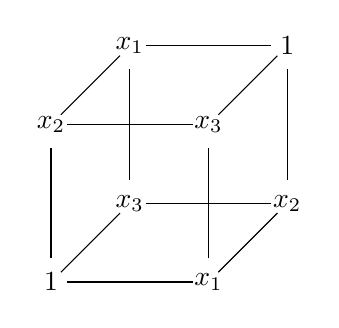
\begin{tikzpicture}
\node at (0,0) {$1$};
\node at (2,0) {$x_1$};
\node at (0,2) {$x_2$};
\node at (2,2) {$x_3$};

\node at (1,1) {$x_3$};
\node at (3,1) {$x_2$};
\node at (1,3) {$x_1$};
\node at (3,3) {$1$};

\draw (0+0.2,0)--(2-0.2,0);
\draw (0+0.2,2)--(2-0.2,2);
\draw (1+0.2,1)--(3-0.2,1);
\draw (1+0.2,3)--(3-0.2,3);

\draw (0,0+0.3)--(0,2-0.3);
\draw (2,0+0.3)--(2,2-0.3);
\draw (1,1+0.3)--(1,3-0.3);
\draw (3,1+0.3)--(3,3-0.3);

\draw (0+0.125,0+0.125)--(1-0.125,1-0.125);
\draw (2+0.125,0+0.125)--(3-0.125,1-0.125);
\draw (0+0.125,2+0.125)--(1-0.125,3-0.125);
\draw (2+0.125,2+0.125)--(3-0.125,3-0.125);

\end{tikzpicture}

\vfill



\begin{thebibliography}{}

\item Amit Ghosh, Peter Sarnak. \\ 
\textbf{Integral points on Markoff type cubic surfaces} \texttt{arXiv:1706.06712}

\item Jean Bourgain, Alex Gamburd, Peter Sarnak. \\
\textbf{Markoff Triples and Strong Approximation} \hspace{30pt}\texttt{arXiv:1505.06411} \\
\textbf{Markoff Surfaces and Strong Approximation: 1} \texttt{arXiv:1607.01530}

\item Ori Parzanchevski, Peter Sarnak. \textbf{Super-Golden-Gates for PU(2)} \texttt{arXiv:1704.02106}

\item J.W.S. Cassels. \\ \textbf{Diophantine Approximation} (Cambridge Tracts in Mathematical Physics, \#45) \\ Cambridge University Press, 1957. 

\item Vladimir Platonov, Andrei Rapinchuk. \\ \textbf{Algebraic Groups and Number Theory}
Academic Press, 1994.

\item Emmanuel Breuillard and Hee Oh (eds.) \textbf{Thin Groups and Superstrong Approximation} 
\texttt{http://library.msri.org/books/Book61/contents.html} Cambridge University Press, 2014.
\end{thebibliography}


\begin{thebibliography}{}

\item Evan O'Dorney
\textbf{Rings of small rank over a Dedekind domain and their ideals} \texttt{arXiv:1508.02777}

\item Takashi Taniguchi, Frank Thorne. \\ 
\textbf{Levels of distribution for sieve problems in prehomogeneous vector spaces} \texttt{arXiv:1707.01850}



\end{thebibliography}


\end{document}